\documentclass[a4paper]{article}

\usepackage{tecnico_relatorio}

\usepackage{textcomp}
\usepackage[hypcap]{caption} % makes \ref point to top of figures and tables
\usepackage{rotating}

\begin{document}
	\trSetImage{img/tecnico_logo}{6cm} % Logotipo do Técnico
	\trSetSubject{Arquitecturas Avançadas de Computadores}
	\trSetType{Laboratório II}
	\trSetTitle{Descrição do Processador \textmu RISC a Funcionar em Pipeline}
	
	\trSetBoxStyle{0.3}
	
	\trSetAuthorNr{3}
	
	\trSetAuthors
		{
		Gonçalo Ribeiro
		
		73294
		}{
		Miguel Costa
		
		73359
		}{
		Rafael Gonçalves
		
		73786
		}
		
	\trSetProfessor{Prof. Leonel Sousa}
	
	\trMakeCover
	
	\tableofcontents
	\pagebreak
	
	\section{Introdução}
	
	Nesta parte do trabalho pretende-se que o processador descrito na primeira parte passe a ter funcionamento em \textit{pipeline}. Como visto nas aulas teóricas isto permitirá aumentar o número de instruções que são executas por ciclo de relógio---IPC.
	
	No entanto, introduzir \textit{pipelining} acarreta problemas que não existiam na versão anterior. É agora preciso ter em conta a existência de conflitos de dados e conflitos de controlo. Para mitigar o impacto destes problemas são implementados circuitos de detecção de conflitos, \textit{forwarding} e previsão dinâmica de saltos.
	
	
	\section{Introdução de Registos de \textit{Pipelining}}
	
	O primeiro passo para garantir o funcionamento em \textit{pipeline} é colocar registos entre os vários andares do processador, i.e.\ introduzir registos entre IF e ID/RF, ID/RF e EX/MEM e entre EX/MEM e WB.
	
	Estes registos já constavam da descrição do processador entregue na primeira parte deste trabalho. Deste modo, relativamente a estes registos bastou fazer com que os seus sinais de \textit{enable} sejam agora controlados pelo próprio processador e não por uma máquina de estados externa, como era feito na primeira parte do trabalho. Na \autoref{fig:circuit_pt1} recorda-se o circuito do processador descrito na primeira parte do projecto.
	
		\begin{figure}[h]
			\centering
			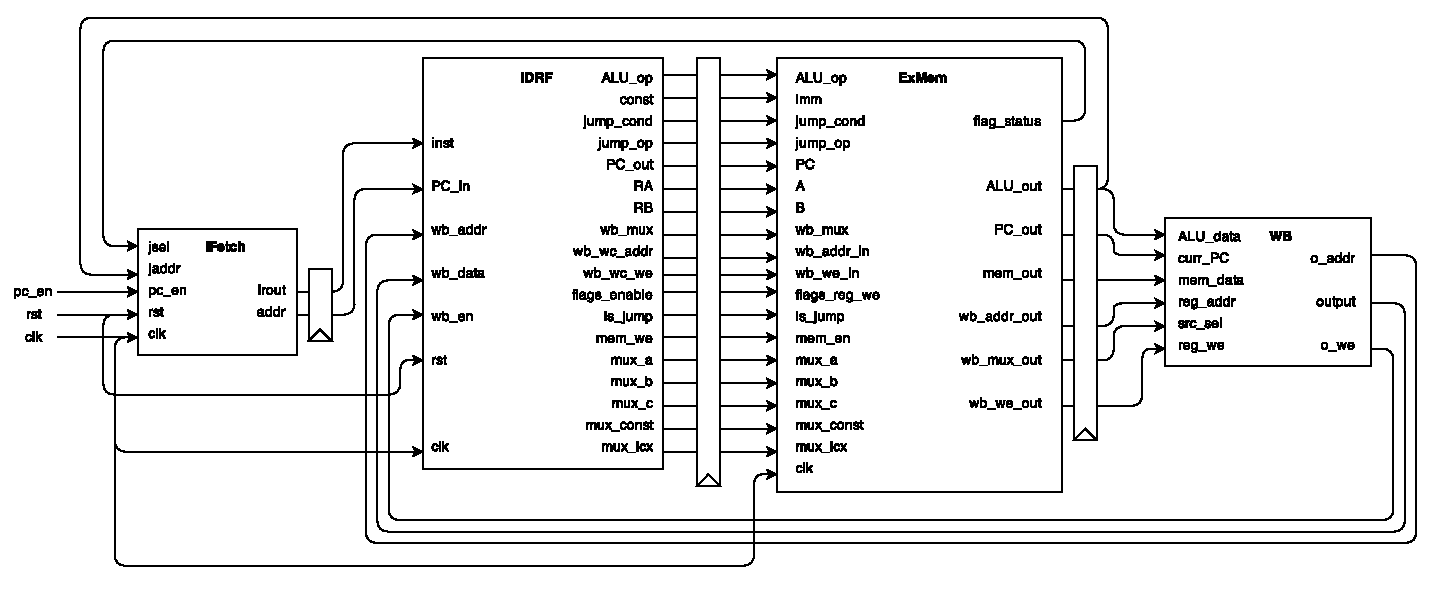
\includegraphics[width=1.\textwidth]{img/circuit_pt1}
			\caption{Circuito do \textmu RISC na primeira parte do trabalho. Podem ser vistos os registo entre andares}
			\label{fig:circuit_pt1}
		\end{figure}
	
	\section{Conflitos de Dados}
	
	\subsection{Detecção}
	
	Não é implementada execução fora de ordem pelo que não existem anti-dependências. Ou seja, esta arquitectura tem apenas o tipo de conflitos de \textit{read after write}---RAW.
	
	Para detectar os conflitos de dados basta, neste caso, verificar se nos andares a seguir ao ID/RF está uma instrução que vá escrever num dos registos lidos pela instrução que está actualmente no ID/RF. Ou seja, existe um conflito de dados se o \textit{enable} do RF estiver activo no andar EX/MEM ou no WB e o endereço do registo que vai ser escrito corresponde a um dos que está a ser lido em ID/RF. Se isto se verificar é feito um \textit{stall} do processador---os andares do ID/RF e IF ficam parados e a instrução em EX/MEM avança para WB.
	
	Na verdade os sinais em WB não são verificados porque a escrita para o RF foi tornada transparente, como descrito em \ref{subsec:RF_write}.
	
	\subsection{Escrita Transparente do \textit{Register File}}
	\label{subsec:RF_write}
	
	Uma forma muito simples de começar a mitigar os conflitos de dados é alterar o flanco em que o \textit{Register Rile} é escrito.
	
	Na primeira parte do trabalho o RF era escrito sempre no flanco de relógio ascendente. Com a introdução do funcionamento em \textit{pipeline}, isto obriga a fazer um \textit{stall} sempre que num mesmo ciclo o WB for escrever num registo R$x$ e em ID/RF estiver a ser feito \textit{fetch} do valor de R$x$.
	
	Para resolver este problema o RF passa a ser escrito no flanco de relógio descendente. Assim, quando R$x$ é lido (no flanco ascendente) o valor de R$x$ já foi actualizado no flanco descendente, pelo que não é necessário atrasar a execução da instrução que está a ler o operando R$x$.
	
	\subsection{\textit{Forwarding}}
	
	Para evitar que o processamento seja atrasado quando é detectado um conflito de dados, implementou-se \textit{forwarding} da saída do andar EX/MEM (antes dos registos) para a saída do andar ID/RF (antes dos registos).
	
	Quando é verificada a existência de um conflito é feita uma substituição do valor lido do RF pelo valor correcto, reencaminhado da saída do EX/MEM. O valor reencaminhado tanto pode ser um resultado da ALU como um valor lido da memória, dependendo do tipo de operação que o EX/MEM está a executar.
	
	Com este \textit{forwarding}, em conjunto com a escrita transparente descrita em \ref{subsec:RF_write}, os conflitos de dados ficam totalmente resolvidos. É de notar que com este método de mitigação deixam de existir \textit{stalls} devidos a conflitos de dados.
	
	\section{Conflitos de Controlo}
	
	\subsection{Detecção}
	
	Os conflitos de controlo resultam das instruções de salto. Quando uma instrução de salto chega ao ID/RF o PC pode já conter um endereço incorrecto. É portanto necessário verificar se o endereço contido no PC permite continuar uma execução correcta do programa. Caso se verifique que o PC contém um valor indesejado, a instrução correspondente a esse endereço é esmagada (\textit{crush}) antes que consiga entrar no ID/RF. Isto é conseguido à custa de fazer um \textit{reset} aos registos entre IF e ID/RF.
	
	Os casos em que é necessário esmagar a instrução são:
	
	\begin{itemize}
		\item o salto é incondicional (inclui  \texttt{JAL} e \texttt{JR}) e o PC não contém o endereço de salto;
		\item o salto é \textit{taken} e o PC não contém o endereço de salto;
		\item o salto é \textit{not taken} e o PC não contém PC + 1.
	\end{itemize}

	Nos casos em que é feito \textit{crush} o PC é actualizado com o endereço correcto, e continua-se a execução do programa.
	

	\subsection{Somador em ID/RF}
	
	Na primeira parte do trabalho, os endereços de salto eram calculados no andar EX/MEM. Caso isso continuasse a ser feito na nova arquitectura com \textit{pipeline}, seria necessário deixar a instrução de salto avançar até EX/MEM e só depois poderia ser verificado se o PC estava a executar a instrução correcta ou se era necessário fazer \textit{crush}.
	
	De forma a antecipar a detecção dos conflitos de controlo adicionou-se um somador ao andar ID/RF. Este somador permite que o endereço de salto seja calculado neste andar, em vez de ser no andar EX/MEM.
	
	\subsection{Previsão Dinâmica de Saltos}
	
	A utilização de previsão dinâmica de saltos permite reduzir a taxa de \textit{crushes} por instrução de salto. A forma de previsão implementada consiste na utilização de um BTB---\textit{branch target buffer}. Pode-se pensar neste componente como um histórico dos efeitos que várias instruções de salto produziram anteriormente: quando de uma instrução de salto resulta um esmagamento, é actualizada a entrada do BTB correspondente à instrução de salto que foi mal prevista. Espera-se assim que das próximas vezes que a instrução for executada exista uma previsão correcta de se o salto deve ser \textit{taken} ou não. Cada previsão correcta é menos um \textit{crush} que é necessário, menos um ciclo de execução perdido.
	
	Os pormenores da BTB implementada são os seguintes:
	
	\begin{itemize}
		\item 8 bits para guardar a \textit{tag} (parte alta do endereço do PC);
		\item 1 bit de validade;
		\item 16 bits para guardar o endereço que se prevê ser o destino do salto.
	\end{itemize}
	
	A BTB tem portanto 256 entradas de 25 bits, o que totaliza 800 bytes.
	
	\section{Testes e Simulações}
		
	\section{Conclusão}

\end{document}








